\documentclass[border=5pt]{standalone}
\usepackage{tikz}
\usepackage{amsmath}
\usetikzlibrary{positioning, arrows.meta, calc, fit, backgrounds}

% --- Color Scheme (Blue-Gray) ---
\definecolor{bgPrimary}{HTML}{DAE8FC}
\definecolor{bgSecondary}{HTML}{E8EEF7}
\definecolor{bgAccent}{HTML}{B3CDE3}
\definecolor{bgInput}{HTML}{F0F4F8}
\definecolor{borderPrimary}{HTML}{6C8EBF}
\definecolor{borderAccent}{HTML}{3A6EA5}
\definecolor{arrowColor}{HTML}{4A6A8A}
\definecolor{textMain}{HTML}{2C3E50}
\definecolor{textLight}{HTML}{7F8C8D}
\definecolor{bgHighlight}{HTML}{FFF3CD}

% --- Styles ---
\tikzset{
  module/.style={
    draw=borderPrimary, fill=bgPrimary, rounded corners=4pt,
    minimum width=2.8cm, minimum height=1.1cm,
    font=\sffamily\small, text=textMain, line width=0.6pt, align=center,
  },
  novelmodule/.style={
    draw=borderAccent, fill=bgAccent, rounded corners=4pt,
    minimum width=2.8cm, minimum height=1.1cm,
    font=\sffamily\small\bfseries, text=textMain, line width=1.0pt, align=center,
  },
  iobox/.style={
    draw=borderPrimary, fill=bgInput, rounded corners=3pt,
    minimum width=2cm, minimum height=0.9cm,
    font=\sffamily\small, text=textMain, line width=0.5pt, align=center,
  },
  stdarrow/.style={
    -{Stealth[length=5pt, width=4pt]}, line width=0.6pt, color=arrowColor,
  },
}

\begin{document}
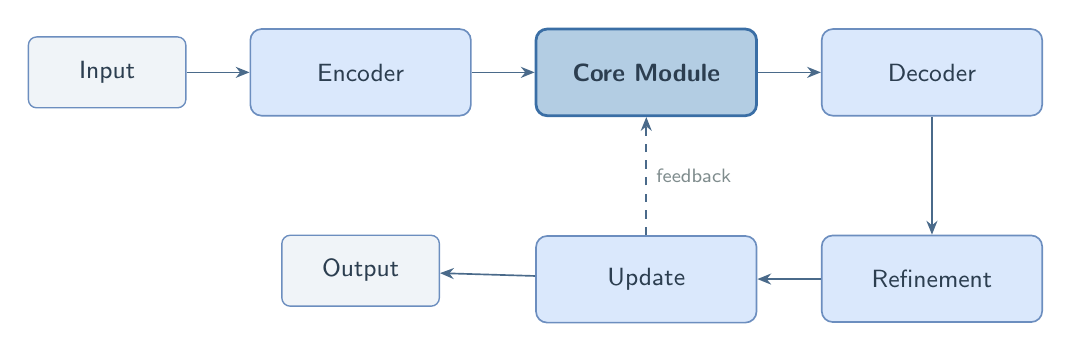
\begin{tikzpicture}

  % --- Top row (left to right): forward pass ---
  \node[iobox]      (input) {Input};
  \node[module,      right=0.8cm of input] (enc) {Encoder};
  \node[novelmodule, right=0.8cm of enc]   (core) {\textbf{Core Module}};
  \node[module,      right=0.8cm of core]  (dec) {Decoder};

  % --- Bottom row (right to left): refinement / feedback ---
  \node[module, below=1.5cm of dec]  (refine)  {Refinement};
  \node[module, below=1.5cm of core] (update)  {Update};
  \node[iobox,  below=1.5cm of enc]  (output)  {Output};

  % --- Top row arrows ---
  \draw[stdarrow] (input) -- (enc);
  \draw[stdarrow] (enc)   -- (core);
  \draw[stdarrow] (core)  -- (dec);

  % --- Turn: top-right to bottom-right ---
  \draw[stdarrow] (dec.south) -- (refine.north);

  % --- Bottom row arrows (right to left) ---
  \draw[stdarrow] (refine) -- (update);
  \draw[stdarrow] (update) -- (output);

  % --- Feedback arrow (bottom to top, optional) ---
  \draw[stdarrow, dashed] (update.north) -- node[right, font=\sffamily\scriptsize, text=textLight] {feedback} (core.south);

\end{tikzpicture}
\end{document}
